\begin{wrapfigure}{R}{0.5\textwidth}
                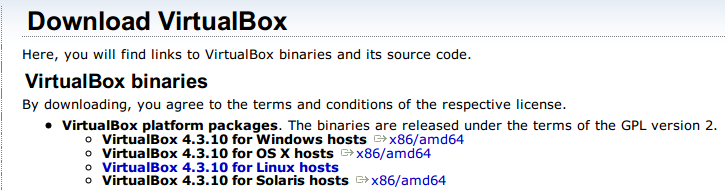
\includegraphics[width=\linewidth]{images/virtualbox_download.png}
\end{wrapfigure}

Alternatywnym sposobem wypróbowania Ubuntu bez instalowania go bezpośrednio na komputerze jest wykorzystanie maszyny wirtualnej. Oprogramowanie to umożliwia uruchomienie systemu operacyjnego zwanego "gościem", jako program działający wewnątrz drugiego systemu, zwanego "gospodarzem". Wiąże się to oczywiście z dużym zapotrzebowaniem na moc obliczeniową procesora oraz pamięć operacyjną. Jeżeli masz przynajmniej 2 gigabajty RAMu, a twój procesor jest nie starszy niż 5 lat (wtedy jest szansa, że będzie zapewniał akcelerację sprzętową dla wirtualizacji) to możesz w ten sposób wypróbować Ubuntu.

Jedną z najpopularniejszych maszyn wirtualnych jest VirtualBox. Udaj się na stronę \href{https://www.virtualbox.org/wiki/Downloads}{virtualbox.org/download} i pobierz instalator VirtualBoksa dla swojego systemu. Zainstaluj pobrany plik w swoim systemie i uruchom program VirtualBox. Przy pierwszym uruchomieniu, program zapyta cię, czy pobrać i zainstalować dodatkowe rozszerzenia od Oracle. Zgódź się.
\clearpage
\begin{center}
        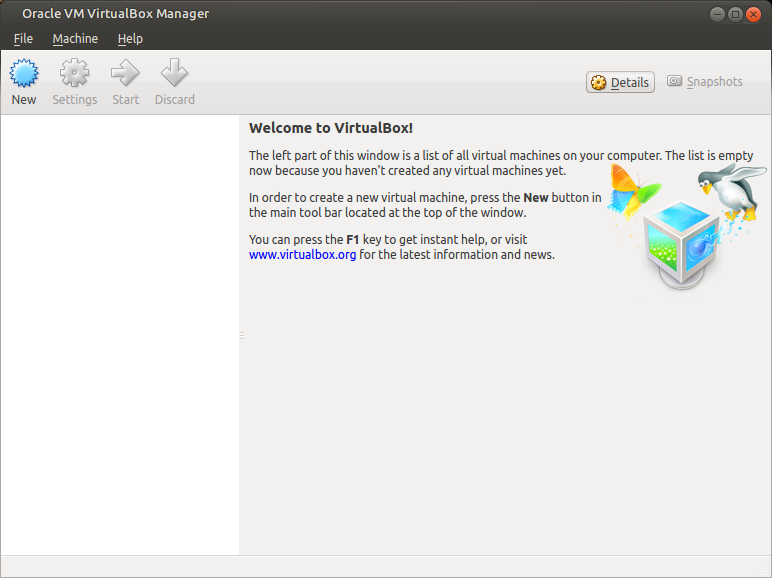
\includegraphics[scale=0.7]{images/virtualbox_main.png}
\end{center}

W oknie głównym programu VirtualBox kliknij na przycisk \textcolor{ubuntu_orange}{New} aby uruchomić kreator maszyny wirtualnej.
\clearpage
\begin{wrapfigure}{r}{0.5\textwidth}
                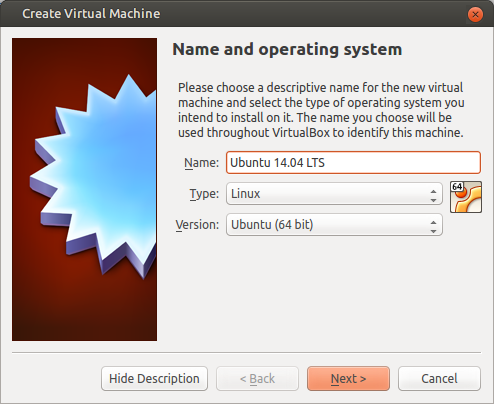
\includegraphics[width=\linewidth]{images/virtualbox_wizard1.png}
\end{wrapfigure}

\begin{itemize}
\item \textcolor{ubuntu_orange}{Name} - Nazwa maszyny wirtualne. Może to być cokolwiek.
\item \textcolor{ubuntu_orange}{Type} - Typ systemu. Ustaw na \textcolor{ubuntu_orange}{Linux}
\item \textcolor{ubuntu_orange}{Version} - Wersja systemu. Ustaw na \textcolor{ubuntu_orange}{Ubuntu (64 bit)}.\\
Uwaga: Architektura wybranego systemu (32/64 bit) musi odpowiadać pobranemu obrazowi instalatora Ubuntu. Dodatkowo należy pamiętać, że na 64 bitowym procesorze (najprawdopodobniej taki posiadasz, jeżeli twój komputer nie jest starszy niż 6 lat) można zainstalować zarówno 64, jak i 32 bitowy system-gościa, natomiast na procesorze 32 bitowym można zainstalować jedynie 32 bitowy system-gość.
\end{itemize}
\begin{flushright}
Kliknij na przycisk \textcolor{ubuntu_orange}{Next} aby przejść dalej.
\end{flushright}

\clearpage
\begin{wrapfigure}{r}{0.5\textwidth}
                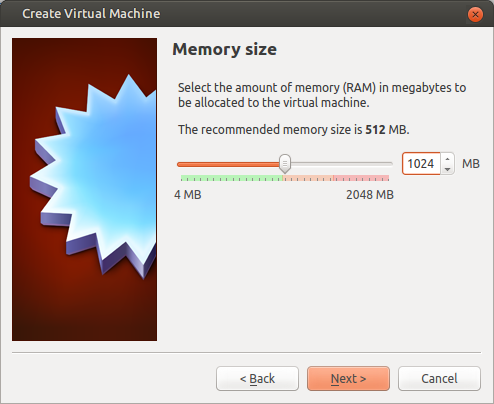
\includegraphics[width=\linewidth]{images/virtualbox_wizard2.png}
\end{wrapfigure}

Na tym ekranie ustaw ilość pamięci operacyjnej twojego komputera, jaką chcesz przeznaczyć dla systemu-gościa. Weź pod uwagę, że ta pamięć zostanie zajęta w momencie uruchomienia maszyny wirtualnej i nie będzie dostępna dla systemu-gospodarza. Nie powinno się przydzielać gościowi więcej niż 50\% zasobów gospodarza. Ubuntu wymaga minimum 512 megabajtów (system plus oprogramowanie) a zdecydowanie lepiej jest przydzielić 1024 megabajty.
Jeżeli w twój komputer posiada tylko 2 gigabajty RAMu, to przydzielając 1 gigabajt gościowi, pozostanie ci tylko 1 gigabajt dla gospodarza. Nie jest to dobre rozwiązanie, gdyż prawdopodobnie będziesz musiał wyłączyć większość programów na systemie gospodarza, aby nie doszło do przepełnienia pamięci operacyjnej. Prawie na pewno będziesz musiał wyłączyć przeglądarkę internetową.
\begin{flushright}
Kliknij na przycisk \textcolor{ubuntu_orange}{Next} aby przejść dalej.
\end{flushright}
\clearpage
\begin{wrapfigure}{r}{0.5\textwidth}
                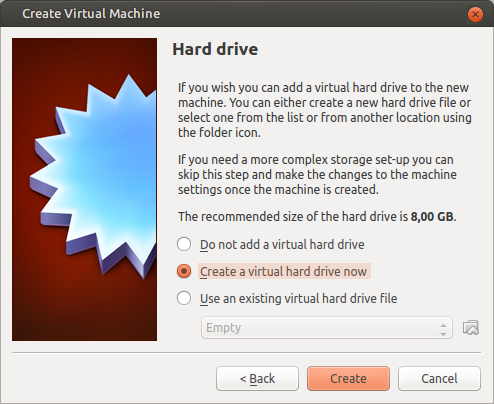
\includegraphics[width=\linewidth]{images/virtualbox_wizard3.png}
\end{wrapfigure}

Ten ekran pozwala skorzystać z już istniejącego wirtualnego dysku twardego lub stworzyć nowy. Ponieważ nie masz jeszcze żadnego takiego urządzenia, wybierz środkowa opcję \textcolor{ubuntu_orange}{Create a virtual hard drive now}.
\begin{flushright}
Kliknij na przycisk \textcolor{ubuntu_orange}{Next} aby przejść dalej.
\end{flushright}
\clearpage
\begin{wrapfigure}{r}{0.5\textwidth}
                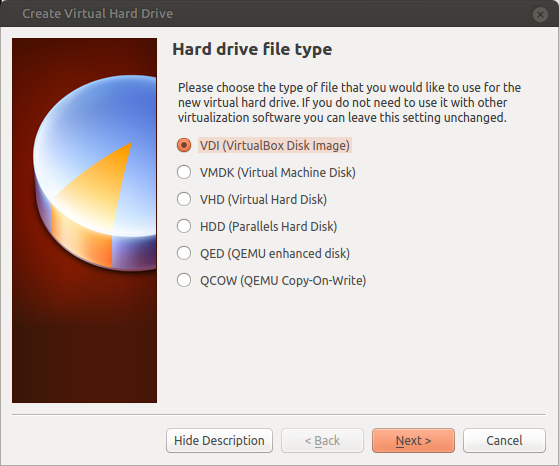
\includegraphics[width=\linewidth]{images/virtualbox_wizard4.png}
\end{wrapfigure}

Na tym ekranie wybierz typ dysku twardego. Wybierz opcję \textcolor{ubuntu_orange}{VDI (Virtual Disk Image)}.
\begin{flushright}
Kliknij na przycisk \textcolor{ubuntu_orange}{Next} aby przejść dalej.
\end{flushright}
\clearpage
\begin{wrapfigure}{r}{0.5\textwidth}
	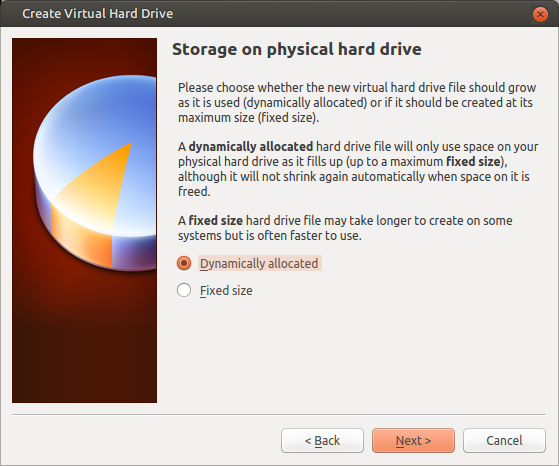
\includegraphics[width=\linewidth]{images/virtualbox_wizard5.png}
\end{wrapfigure}

Wybierz pomiędzy dyskiem tworzonym dynamicznie a dyskiem o stałym rozmiarze.
\begin{itemize}
\item \textcolor{ubuntu_orange}{Dynamically allocated} - Taki wirtualny dysk twardy nie zajmuje całego przydzielonego miejsca a jedynie tyle ile wynosi suma rozmiaru plików na nim zapisanych. Nawet jeżeli stworzysz dysk o pojemności 100 gigabajtów, to po instalacji Ubuntu będzie on zajmował tylko trochę ponad 6 gigabajtów na systemie-gospodarzu. Wybierz tę opcję.
\item \textcolor{ubuntu_orange}{Fixed size} - Taki dysk twardy zawsze zajmuje tyle miejsca na systemie-gospodarzu ile zostało zadeklarowane. Jeżeli stworzysz 100 gigabajtowy dysk wirtualny, to na twoim komputerze pojawi się 100 gigabajtowy plik z maszyną wirtualną. Tworzenie takiego dysku też trwa dłuższą chwilę, gdyż dużo danych musi zostać zapisanych na dysk.
\end{itemize}
\begin{flushright}
Kliknij na przycisk \textcolor{ubuntu_orange}{Next} aby przejść dalej.
\end{flushright}
\clearpage
\begin{wrapfigure}{r}{0.5\textwidth}
                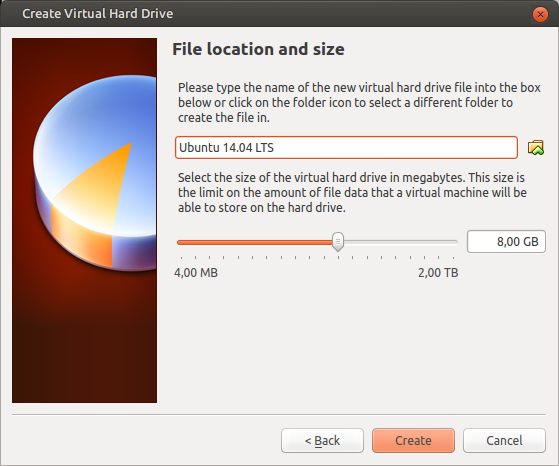
\includegraphics[width=\linewidth]{images/virtualbox_wizard6.png}
\end{wrapfigure}

Na tym ekranie możesz wybrać rozmiar dysku twardego. Korzystając z suwaka możesz wybrać żądany rozmiar. Ubuntu 14.04 LTS wymaga przynajmniej 6.2 gigabajta, górną granicą są tylko możliwości VirtualBoksa (2 terabajty). W celach testowych stwórz dysk o rozmiarze przynajmniej 25 gigabajtów.

Kliknij na przycisk \textcolor{ubuntu_orange}{Create} aby stworzyć dysk i zakończyć działanie kreatora.

\clearpage
\begin{center}
	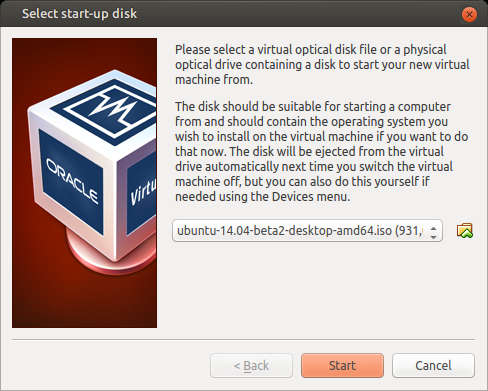
\includegraphics[width=\linewidth]{images/virtualbox_start.png}
\end{center}

Twoja maszyna wirtualna dla Ubuntu jest gotowa. W głównym oknie programu VirtualBox jest teraz dostępna. Kliknij na nią i z paska narzędziowego wybierz \textcolor{ubuntu_orange}{Start}. Alternatywnym sposobem uruchomienia maszyny wirtualnej jest dwukrotne kliknięcie na jej ikonie. Twoim oczom ukaże się okno jak na rysunku powyżej. Kliknij na żółtą ikonę folderu i wskaż pobrany wczesnej obraz instalatora systemu Ubuntu (plik .iso). Kliknij \textcolor{ubuntu_orange}{Start} aby uruchomić maszynę wirtualną. Instalacja na maszynie wirtualnej przebiega tak samo jak w rzeczywistości. Przejdź do sekcji \ref{instalacja_uruchomienie}: "Uruchomienie instalatora BIOS".

Kiedy po zakończeniu instalacji zostaniesz poproszony o wyjście płyty instalatora z napędu to z paska menu maszyny wirtualnej wybierz \textcolor{ubuntu_orange}{Devices -> Cd/DVD Devices -> Remove disk from virtual drive}.

Żeby móc się cieszyć w pełni sprawną maszyną wirtualną należy doinstalować w systemie-gościu \textcolor{ubuntu_orange}{Używanie x86 virtualization solution - guest addition module source for dkms z virtualbox-guest-dkms (własnościowy)} zgodnie z instrukcją zawartą w \ref{pierwsze_uruchomienie_aktualizacja_instalacja}: "Instalacja dodatkowych sterowników".
\clearpage
